\documentclass[a4paper, 10pt, twocolumn]{article}

% Configuration {{{
\usepackage[utf8]{inputenc}
\usepackage[T2A]{fontenc} % T1 for English
\usepackage[english, russian]{babel}

\usepackage{enumitem}
\setlist{nolistsep}
\usepackage{mathtools}
\usepackage{xcolor}
\definecolor{dimblue}{HTML}{1010aa}
\usepackage[
	colorlinks=true, 
	allcolors=dimblue
]{hyperref}
\usepackage[
	vmargin=1in,
	hmargin=.8in
]{geometry}
\setlength{\columnsep}{.25in}
%\usepackage[nospread]{flushend}
\usepackage{cuted}
\linespread{1.3}
\usepackage{indentfirst}
\usepackage{graphicx}
\usepackage[multidot]{grffile}
\usepackage[labelsep=period]{caption}

\usepackage{titlesec}
\titleformat{\section}[hang]{\bf\centering}{\thesection.}{.5em}{}[]
\def\thesection{\Roman{section}}
\def\thefootnote{\fnsymbol{footnote}}

\usepackage{ifthen}
\newboolean{articletitles}
\setboolean{articletitles}{true}
\newboolean{italicNames}
\setboolean{italicNames}{false}
\newboolean{italicTitles}
\setboolean{italicTitles}{true}
% }}}

\begin{document}

% Title {{{
\begin{strip}
\begin{center}
\vskip-2.4\baselineskip
{\large\textbf{Физика тяжелых адронов}}
\vskip.3\baselineskip
{Керим Гусейнов\footnotemark}
\vskip.3\baselineskip
\today
\end{center}
\end{strip}
\footnotetext{\href{mailto:guseynovkerim@gmail.com}{guseynovkerim@gmail.com}}
% }}}

\section{Введение}
% {{{

В физике частиц стандартная модель на данный момент является самой 
успешной теорией и с большой точностью описывает многие процессы 
и реакции. Однако существуют глобальные проблемы, объяснить которые 
в рамках СМ не удается. Список таких проблем включает
\begin{itemize}
	\item осцилляции нейтрино,
	\item барионную асимметрию вселенной,
	\item темную материю,
	\item стабильность массы бозона Хиггса из-за петлевых поправок,
	\item иерархию масс фундаментальных частиц.
\end{itemize}
Кроме того, СМ не притрагивается к объяснению гравитации и даже 
несовместима с общей теорией относительности -- наиболее действенной 
теорией гравитации из существующих. Это означает, что СМ не может быть 
окончательной теорией, описывающей мир вокруг нас.

Однако СМ описывает эксперимент с большой точностью, и любые новые 
теории должны описывать с не меньшей, а значит, их можно искать в виде 
расширений Стандартной модели. Возможных расширений со стороны теории 
было предложено немало, но даже самые грандиозные и громкие, теории 
великого объединения и суперсимметрии, до сих пор не находят 
подтверждения в эксперименте.

Всю физику, выходящую за рамки СМ, называют новой физикой. Поиски новой 
физики~-- одна из главных задач трех из четырех крупных экспериментов 
Большого адронного коллайдера: ATLAS, CMS и LHCb. ATLAS и CMS подходят 
к этой задаче в основном со стороны грубой силы: в них ведутся поиски 
прямого рождения частиц, составляющих новую физику. Возможен еще один 
путь -- непрямой. В этом случае изучаются эффекты воздействия новой 
физики на какие-либо процессы, возможно даже разрешенные в СМ. 
Наилучшим образом, конечно, влияние будет заметно при изучении 
процессов, вероятность которых в СМ хотя бы подавлена. Чем больше узлов 
и частиц содержит диаграмма Фейнмана какого-либо процесса в СМ, тем 
более вероятно появление новых частиц в диаграмме, а значит и вклад 
новой физики. Именно поэтому и появляется интерес к реакциям, редко 
происходящим в Стандартной модели. Например, к редким распадам. 
Сравнение вероятностей, продиктованной СМ и полученной в эксперименте, 
и поиск отклонений от СМ дают физикам улики, указывающие на правильное 
направление к новой теории.

С другой стороны, интерес к Стандартной модели не угасает, 
и потребность в более точных измерениях и вычислениях параметров СМ все 
так же велика. Касательно адронных коллайдеров и физики адронов 
в целом, наибольший интерес представляют прецезионные измерения 
параметров бозона Хиггса и матрицы ККМ. Очевидно, последнее затрагивает 
физику адронов гораздо больше. Матрица Кабиббо-Кобаяши-Маскава 
определяет вероятности слабых переходов между кварками, 
а следовательно, и слабых распадов адронов. Кроме того, комплексная 
фаза в ней служит единственным источником нарушения 
$CP$\babelhyphen{nobreak}четности в Стандартной модели.

Таким образом, изучение распадов адронов, содержащих один или два $c$- 
или $b$-кварка, предоставляет многочисленные сценарии проверки СМ 
и уточнения множества её параметров.

% }}}

\section{Детектор LHCb}
% {{{

\begin{figure*}% {{{
	\centering
	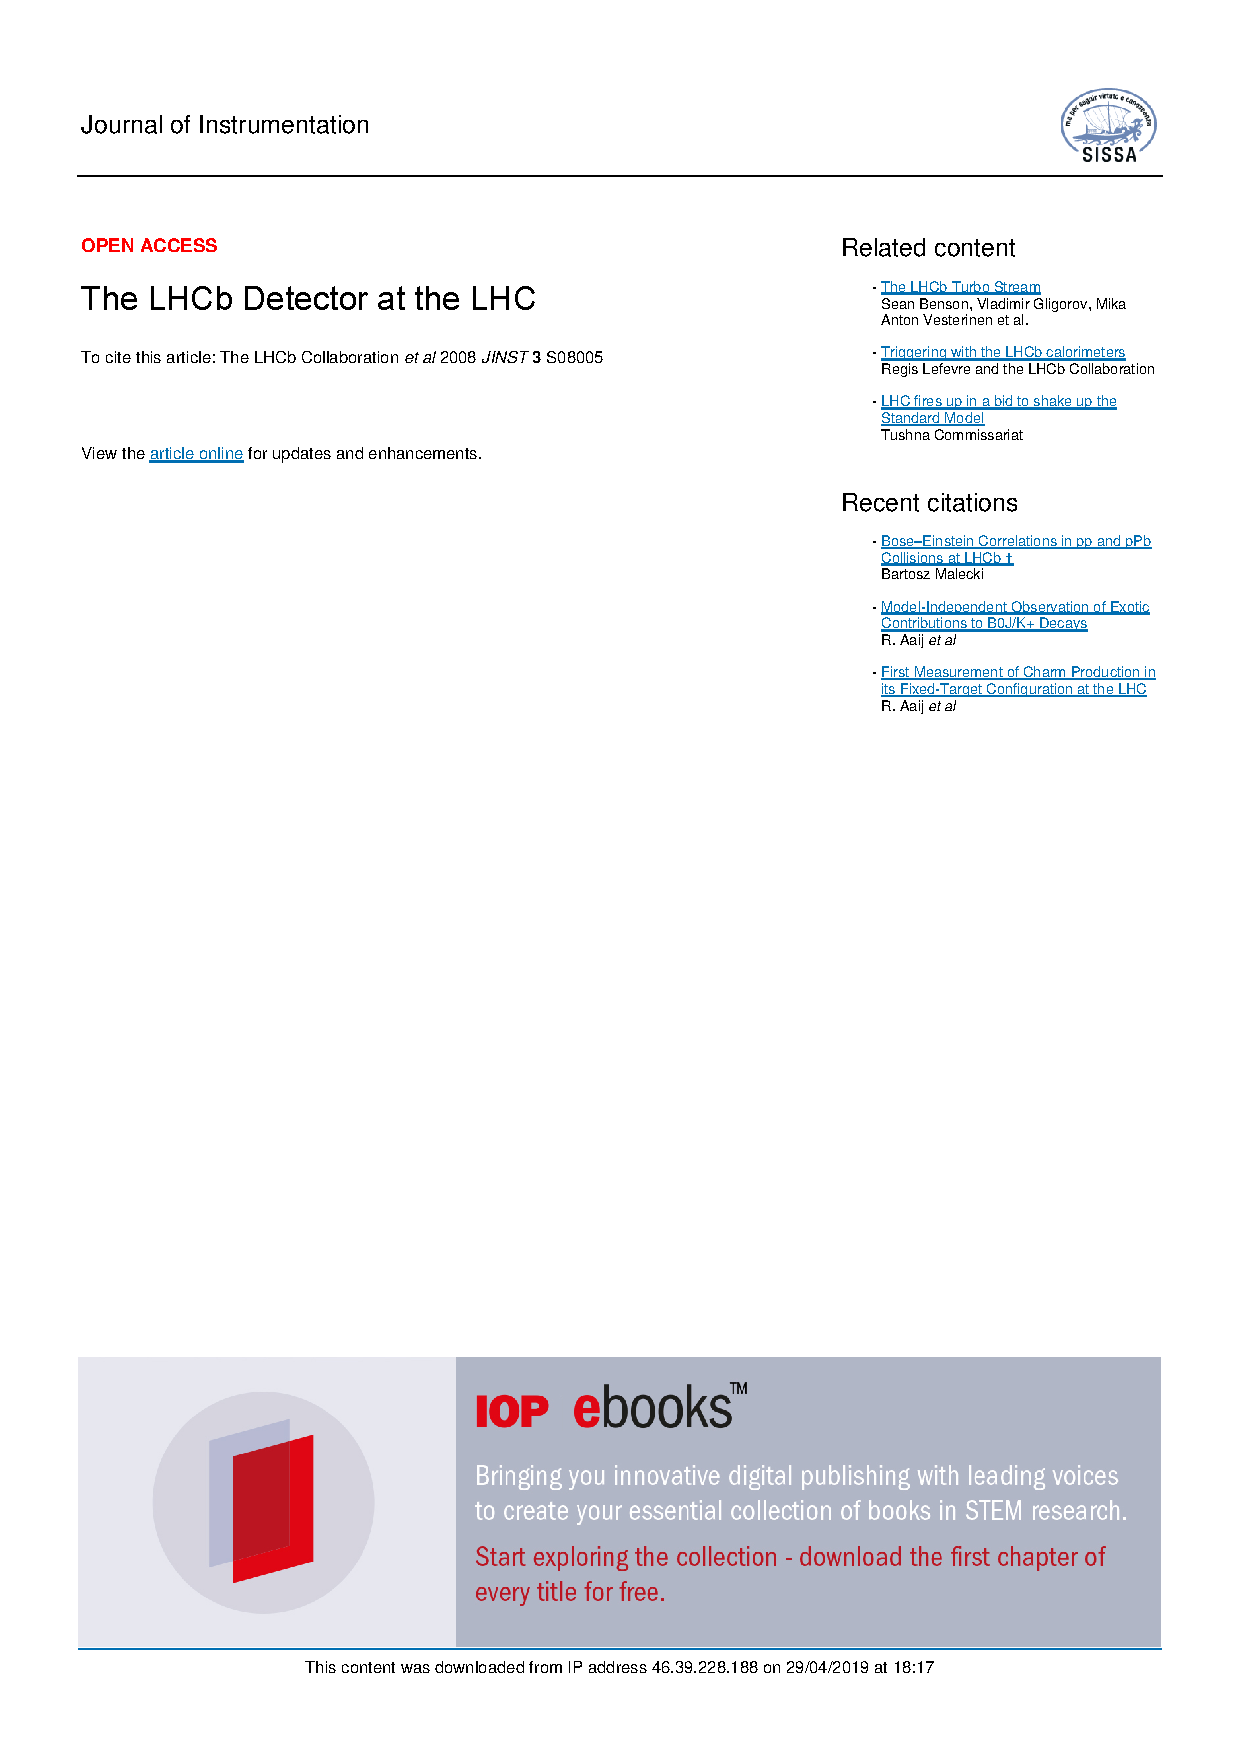
\includegraphics[width=.67\linewidth]{figures/LHCb-detector}
	\caption{Общий вид детектора LHCb и его частей.}
	\label{fig:detector}
\end{figure*}% }}}

Детектор LHCb~\cite{LHCb-detector} расположен на Большом адронном 
коллайдере -- самом мощном ускорителе в истории физики частиц. Высокие 
энергии, достигаемые протонными пучками, и большие светимости позволяют 
подробно изучать прежде даже не наблюдавшиеся процессы. Сам детектор 
LHCb, в свою очередь, имеет ряд отличительных особенностей, позволяющих 
производить специфические эксперименты и с большей точностью наблюдать 
за распадами тяжелых адронов. Можно назвать две основные особенности. 
Во-первых, высокоточный вершинный детектор (vertex locator), 
расположенный вблизи точки соударения протонов, позволяющий определять 
вершины распадов короткоживущих частиц~-- $b$- и $c$-адронов. 
А во-вторых, систему идентификации частиц, основанную на черенковских 
детекторах (RICH1, RICH2). Важно отметить, что остальные два упомянутых  
эксперимента БАК не имеют какой-либо системы идентификации частиц 
вообще. Общий вид детектора представлен на рисунке~\ref{fig:detector}.

Для корректной работы аппаратуры детектора LHCb пучки протонов, 
в отличие от ATLAS и CMS, намеренно формируются менее плотными, чтобы 
не создавать излишних шумов и учитывать мертвое время суб-детекторов. 
Это, конечно, уменьшает получаемую светимость, но позволяет проводить 
более тонкие анализы распадов.

% }}}

\section{Нейтральные $D$, $B$, $B_s$ мезоны}
% {{{

Среди адронов мезоны выделяются тем, что являются собственными 
античастицами. Нейтральные мезоны выделяются еще сильнее, поскольку 
допускают переходы между частицей и античастицей, называемые 
смешиванием. Суть процесса в том, что если в квантовой системе 
присутствуют два уровня и возможен переход между ними, то эти уровни, 
очевидно, не являются решениями стационарного уравнения. Вместо двух 
``старых'' уровней возникают два других, слегка отличающихся друг от 
друга энергией. С точки зрения кварков, мезоны и их массы покоя 
и являются такими состояниями. Однако, смешивание нейтральных мезонов 
обусловлено слабым взаимодействием, а сильное воспринимает их все так 
же в виде ``старых'' состояний. Таким образом, мезон рождается 
в сильном взаимодействии, затем путешествует самостоятельно и, находясь 
под влиянием слабого взаимодействия, раскладывается по его собственным 
векторам, а когда вновь встречается с адроном, возвращается в старый 
базис. Поскольку массы состояний не совпадают, при эволюции слабых 
собственных векторов со временем (или же с пройденным расстоянием) 
возникают осцилляции между частицей и античастицей. Частота этих 
осцилляций зависит от разности масс и позволяет её измерить с большой 
точностью.

Смешивание нейтральных мезонов, очевидно, затрагивает тему переходов 
кварков между собой, а значит и матрицу ККМ. Впервые смешивание 
наблюдалось для $K$ мезонов, состоящих из $\bar{s}d$ или $s\bar{d}$. 
Соответствующие диаграммы Фейнмана представлены на 
рисунке~\ref{fig:kaon-mixing}. Нейтральные $K^0$ и $\bar{K}^0$ 
смешиваются в короткоживущий $K_S$ и долгоживущий $K_L$. Время жизни 
последнего достаточно велико для наблюдения осцилляций. Состояния $K_L$ 
и $K_S$ отличаются также $CP$-четностью, у первого она равна $-1$, 
а у второго -- $+1$, что дает им распады на три пиона и два пиона 
соответственно. Но существует небольшая вероятность распада $K_L \to 
2\pi$, которая и свидетельствует о нарушении 
$CP$-четности~\cite{kaon-CP-violation}. Осцилляции нейтральных каонов 
свидетельствуют о разности масс $\Delta m = 5.293 \pm 0.009 
\text{~нс}^{-1}$~\cite{kaon-oscillations}.

\begin{figure}% {{{
	\centering
	\includegraphics[width=\linewidth]{figures/K-mixing}
	\caption{Диаграммы Фейнмана, обеспечивающие смешивание нейтральных каонов.}
	\label{fig:kaon-mixing}
\end{figure}% }}}

Аналогично себя ведут и более тяжелые нейтральные мезоны $D$, $B$ 
и $B_s$. Их смешивания имеют особенности. $D$-мезоны, содержащие 
$c$-кварк, распадаются настолько быстро, что осцилляции уловить 
практически невозможно. Они были открыты лишь в 2016 году коллаборацией 
LHCb~\cite{D-oscillations}. Прямое $CP$ нарушение, связанное с этими 
мезонами, было найдено совсем недавно~\cite{D-CP-violation}. Осцилляции 
$B$-мезонов были найдены уже давно, а LHCb внес вклад в изучение $CP$ 
нарушения~\cite{B-CP-violation}. Особенностью $B_s$ мезонов является 
чрезвычайно большая частота осцилляций $\Delta m_s = 17.768 \pm 
0.024\text{~пс}^{-1}$~\cite{Bs-oscillations} по сравнению с $\Delta m_d 
= 0.5064 \pm 0.0019\text{~пс}^{-1}$~\cite{B-oscillations} для $B$ 
мезонов и уже названным числом для каонов.

% }}}

\section{Матрица Кабиббо-Кобаяши-Маскава}
% {{{
\def\peakx{\bar{\rho}}
\def\peaky{\bar{\eta}}

Матрица Кабиббо-Кобаяши-Маскава определяет вероятности перехода между 
кварками путем испускания $W$-бозона. Например, компонента $V_{ub}$ 
определяет матричный элемент процесса $b \to u W^-$. Матрица ККМ 
содержит 9 комплексных чисел, то есть 18 параметров. В рамках СМ она 
должна быть унитарной, что уменьшает количество параметров до 9. Среди 
них содержится 5 ненаблюдаемых фаз. То есть в итоге остаются 
4 физически значимых параметра: три угла смешивания и одна фаза. 
Значения этих параметров принято изображать в виде так называемого 
треугольника унитарности. Двум вершинам треугольника приписываются 
координаты $(0,0)$ и $(1,0)$, координаты третьей вершины 
$(\peakx,\,\peaky)$ задаются формулами
$$ \sqrt{\peakx^2 + \peaky^2} = \left| \frac{V_{ud} V_{ub}^*}{V_{cd} V_{cb}^*} \right|, \quad
\sqrt{(1-\peakx)^2 + \peaky^2} = \left| \frac{V_{td} V_{tb}^*}{V_{cd} V_{cb}^*} \right|, $$
а углы $\alpha, \, \beta, \, \gamma$ -- формулами
$$
\alpha = \mathrm{arg}\left(-\frac{V_{td} V_{tb}^*}{V_{ud} V_{ub}^*}\right),
\quad
\beta  = \mathrm{arg}\left(-\frac{V_{cd} V_{cb}^*}{V_{td} V_{tb}^*}\right),
$$$$
\gamma = \mathrm{arg}\left(-\frac{V_{ud} V_{ub}^*}{V_{cd} V_{cb}^*}\right).
$$ 
Экспериментальные измерения компонент матрицы комбинируют и изображают 
на едином графике, как показано на рисунке~\ref{fig:triangle}. Удобство 
и иллюстративность в том, что видно, как разные методы измерения 
параметров матрицы согласуются между собой, образуя вершину 
треугольника. Отсутствие согласия указывало бы на наличие новой физики 
и иные источники $CP$ нарушения. В рамках СМ, чем больше площадь 
треугольника, тем сильнее нарушена $CP$-четность.

\begin{figure}% {{{
	\centering
	\includegraphics[width=\linewidth]{figures/triangle}
	\caption{Треугольник унитарности матрицы ККМ.}
	\label{fig:triangle}
\end{figure}% }}}

Различные буквы на рисунке соответствуют разным физическим процессам. 
$\varepsilon_K$ соответствует распаду $K_L$ мезона на два 
пиона~\cite{kaon-CP-violation-new}. Угол $\beta$ наиболее точно 
определялся из распадов нейтральных $B$-мезонов на $J/\psi 
K_S$~\cite{B-CP-violation}. Углы $\alpha$ и $\gamma$ не имеют таких же 
четких аналогий, а остальные обозначения очевидны из уже написанных 
в этом и предыдущем разделах.

% }}}

\section{Экзотические кварковые состояния}
% {{{

Кварковая модель, вводя цвет, разрешает существование лишь синглетных 
по цвету состояний, то есть мезонов, барионов и антибарионов. Однако 
если назвать адроны атомами, то возможно и существование молекул, ведь 
и они будут цветовыми сигнлетами. Их существование довольно спорно, но 
несомненно вызывает интерес и стимулирует проведение соответствующих 
анализов.

\begin{figure}[b!]% {{{
	\centering
	\includegraphics[width=\linewidth]{figures/Jpsi-p-Dalitz}
	\caption{Диаграмма Далица распада $\Lambda_b^0 \to J/\psi p K^-$.}
	\label{fig:Jpsip-Dalitz}
\end{figure}% }}}

Наиболее громким было обсуждение пентакварковых состояний, 
наблюдавшихся в системе $J/\psi p$. Сначала считали, что присутствуют 
пентакварки с массами 4380 и 4450~МэВ. Затем, последний резонанс 
расщепился на два разных с массами 4440 и 4457~МэВ, а масса легкого 
уменьшилась до 4312~МэВ. Новейший анализ, проведенный на основе всех 
данных, собранных LHCb за Run~1 и Run~2, представлен 
в~\cite{pentaquark}. В нем, как и во всех других анализах на эту тему, 
рассматривается распад $\Lambda_b^0 \to J/\psi p K^-$. Соответствующая 
диаграмма Далица представлена на рисунке~\ref{fig:Jpsip-Dalitz}. Как 
видно, она имеет довольно нетривиальную структуру. Пики в системе 
$pK^-$ обусловлены странными резонансами, а пики в системе $J/\psi p$ 
как раз вызывают интерес. Они свидетельствуют о присутствии связанных 
состояний протона и легчайшего чармония, которые можно интерпретировать 
двумя способами. В случае сильной связи все пять кварков находятся 
близко друг к другу и взаимодействуют глюонами, а в случае слабой связи 
кварки группируются в мезон и барион и взаимодействуют аналогично 
нуклонам в ядре. В анализе распределение масс $J/\psi p$ 
перевзвешивается для лучшего выделения сигнала. Результат показан на 
рисунке~\ref{fig:Jpsip-mass}. Со стороны теории найденным массам лучше 
всего соответствуют связанные состояния $\overline{D}^0\Sigma_c^+$ 
и $\overline{D}^{*0}\Sigma_c^+$, имеющие кварковую структуру 
$u\bar{c}$-$cud$.

\begin{figure}% {{{
	\centering
	\includegraphics[width=\linewidth]{figures/Jpsi-p-mass}
	\caption{Взвешенное распределение масс $J/\psi p$ в распаде $\Lambda_b^0 \to J/\psi p K^-$.}
	\label{fig:Jpsip-mass}
\end{figure}% }}}

Кроме того, недавно был проведен подробный амплитудный анализ распада 
$B^+\to D^+ D^- K^+$, выявивший возможное существование тетракварковых 
состояний в системе $D^-K^+$~\cite{tetraquark}. Однако количества 
событий на данный момент значительно уступают обсуждавшемуся пентакварку.

% }}}

\section{Адронная спектроскопия}
% {{{

Побочной задачей эксперимента LHCb оказывается адронная спектроскопия. 
Я говорю побочной, поскольку измерения на адронном коллайдере, 
разумеется, уступают по точности измерениям с пучками электронов. 
Выигрыш адронных коллайдеров в колоссальном увеличении энергии, 
позволяющем изучать тяжелые адроны. Однако адронная спектроскопия, как 
и все остальное, интересна в сравнении с теорией. Теория здесь очень 
непростая, все расчеты КХД производятся на решетках и требуют больших 
вычислительных мощностей и затрат времени. И чем выше энергия, тем 
более мелкий шаг решетки требуется. В результате теория работает лишь 
с относительно легкими адронными резонансами, в основном даже только со 
странным кварком. И энергетический выигрыш БАК в этом вопросе не 
помогает.

\begin{figure}[p!]% {{{
	\centering
	\includegraphics[width=\linewidth]{figures/xicc}
	\caption{Наблюдение распадов $\Xi_{cc}^{++}\to\Xi_c^+\pi^+$ и $\Xi_{cc}^{++} \to \Lambda_c K^-\pi^+\pi^+$ по инвариантной массе конечных частиц.}
	\label{fig:xicc}
\end{figure}% }}}

\begin{figure}[p!]% {{{
	\centering
	\includegraphics[width=\linewidth]{figures/Bcstar}
	\caption{Распределение разности масс $\Delta M = M(B_c^+\pi^+\pi^-) - M(B_c^+)$.}
	\label{fig:Bcstar}
\end{figure}% }}}

Однако с другой стороны, большие энергии БАК в паре с высокой точностью 
детектора LHCb позволяют открывать крайне редко образующиеся тяжелые 
частицы и подробно их изучать. Наилучшими примерами являются недавние 
наблюдения дважды очарованной частицы $\Xi_{cc}^{++}$~\cite{Xicc++} 
и прелестно-очарованного мезонного резонанса $B_c^{*+}$~\cite{Bcstar}. 
Эти частицы видны в качестве резонансов в распределениях инвариантных 
масс продуктов их распада, как показано на рисунках~\ref{fig:xicc} 
и~\ref{fig:Bcstar} соответственно. На рисунке~\ref{fig:Bcstar} помимо 
резонанса $B_c^*(2^3S_1)^+$, который имеет достаточную статистическую 
значимость, также видно возможное состояние $B_c(2^1S_0)^+$.

% 13 July 2019: Observation of two new beauty baryon particles.

Кроме того, адронная спектроскопия необходима для полного понимания 
происходящих в распадах процессов и в частности для правильного их 
моделирования. Такие анализы чаще всего не являются открытием частиц, 
поскольку появляющиеся в цепочках распадов резонансы легче $b$-адронов 
и в большом количестве были открыты и изучены на B-фабриках Belle 
и BaBar. Подобные работы имеют в основном техническую значимость. 
Например, при изучении многочастичных распадов большое влияние имеют 
эффективности регистрации и восстановления частиц. Определить их 
с приличной точностью предельно сложно, и поэтому рассматривают 
относительные вероятности процессов. Чем ближе процессы друг к другу 
кинематически, тем слабее окажется вклад эффективностей в результат, 
а следовательно, и систематическая погрешность определяемой величины. 
Большой интерес представляют многочастичные распады, а для их изучения 
приходится последовательно рассматривать все более и более сложные 
процессы. Например, на основе анализа распада $\Lambda_b^0 \to 
\Lambda_c^+ \pi^-$ был измерен многочастичный распад $\Lambda_b^0 \to 
\Lambda_c^+ \pi^-\pi^+\pi^-$. А на основе последнего возможно изучение 
распада $\Lambda_b^0 \to D^+ p \pi^-\pi^-$. А он, в свою очередь, 
позволяет измерять распады $\Xi_b$. Кроме того, при изучении процесса 
$\Lambda_b^0 \to \Lambda_c^+ 3\pi$ был выделен целый ряд промежуточных 
очарованных резонансов $\Lambda_c^{*+}$, $\Sigma_c^{*0}$, 
$\Sigma_c^{*++}$~\cite{LbtoLc3pi}, очевидно, влияющих на кинематику 
исходной реакции.

% }}}

\section{Вывод}
% {{{

Физика тяжелых адронов на БАК и других ускорителях позволяет с высокой 
точностью определять массы адронов, изучать каналы их распада 
и измерять их вероятности. Она является хорошей экспериментальной 
проверкой феноменологических моделей адронов, описывающих реакции 
и распады без углубления в КХД.

Редкие распады и предельно точные измерения позволяют проверять 
Стандартную модель и уточнять ее параметры. А экзотические кварковые 
состояния, появляющиеся в экспериментах последние годы, иллюстрируют, 
как много новых явлений нам еще предстоит открыть.

% }}}

\bibliographystyle{local}
\bibliography{refs.bib}

\end{document}
